\documentclass[aspectratio=169,11pt]{beamer}

% TEMA Y COLORES
\usetheme{Madrid}
\usecolortheme{whale}

\definecolor{primaryblue}{RGB}{0,102,153}
\definecolor{accentgreen}{RGB}{0,128,0}
\definecolor{accentorange}{RGB}{204,102,0}
\definecolor{darkgray}{RGB}{64,64,64}

\setbeamercolor{palette primary}{bg=primaryblue,fg=white}
\setbeamercolor{palette secondary}{bg=primaryblue!80,fg=white}
\setbeamercolor{palette tertiary}{bg=primaryblue!60,fg=white}
\setbeamercolor{structure}{fg=primaryblue}
\setbeamercolor{block title}{bg=primaryblue,fg=white}
\setbeamercolor{block body}{bg=primaryblue!10}
\setbeamercolor{block title example}{bg=accentgreen,fg=white}
\setbeamercolor{block body example}{bg=accentgreen!10}
\setbeamercolor{block title alerted}{bg=accentorange,fg=white}
\setbeamercolor{block body alerted}{bg=accentorange!10}

% PAQUETES
\usepackage[utf8]{inputenc}
\usepackage[T1]{fontenc}
\usepackage{amsmath,amssymb}
\usepackage{booktabs}
\usepackage{tikz}
\usepackage{pgfplots}
\usepackage{listings}
\usepackage{multicol}

\pgfplotsset{compat=1.17}

% CÓDIGO PYTHON
\lstdefinestyle{pythonstyle}{
    language=Python,
    basicstyle=\ttfamily\footnotesize,
    keywordstyle=\color{blue}\bfseries,
    stringstyle=\color{red},
    commentstyle=\color{accentgreen}\itshape,
    frame=single,
    breaklines=true,
    showstringspaces=false,
    backgroundcolor=\color{gray!10}
}

% NAVEGACIÓN Y PIE DE PÁGINA
\setbeamertemplate{navigation symbols}{}
\setbeamertemplate{footline}{
    \leavevmode%
    \hbox{%
        \begin{beamercolorbox}[wd=.333333\paperwidth,ht=2.25ex,dp=1ex,center]{author in head/foot}%
            \usebeamerfont{author in head/foot}Matemáticas Financieras
        \end{beamercolorbox}%
        \begin{beamercolorbox}[wd=.333333\paperwidth,ht=2.25ex,dp=1ex,center]{title in head/foot}%
            \usebeamerfont{title in head/foot}Sesión 9
        \end{beamercolorbox}%
        \begin{beamercolorbox}[wd=.333333\paperwidth,ht=2.25ex,dp=1ex,right]{date in head/foot}%
            \usebeamerfont{date in head/foot}\insertframenumber{} / \inserttotalframenumber\hspace*{2ex}
        \end{beamercolorbox}}%
    \vskip0pt%
}

\title[Sesión 9]{VPN y TIR}
\subtitle{Evaluación de proyectos de inversión}
\author{Matemáticas Financieras}
\institute{Valor del Dinero en el Tiempo}
\date{Semana 5 | Clase 1 | Duración: 1h 50min}

\begin{document}

% ===========================================
% SECCIÓN 1: PORTADA Y CONTENIDO
% ===========================================

\begin{frame}
    \titlepage
\end{frame}

\begin{frame}{Contenido de la Sesión}
    \tableofcontents
\end{frame}

% ===========================================
% SECCIÓN 2: INTRODUCCIÓN
% ===========================================
\section{Introducción}

\begin{frame}{Conexión con la Sesión Anterior}
    \begin{block}{Sesión 8: Valuación de Bonos}
        Valuamos bonos con flujos fijos (cupones) usando VP y calculamos el YTM (tasa que iguala precio con VP de flujos).
    \end{block}

    \pause
    \vspace{0.3cm}

    \begin{alertblock}{Hoy: Proyectos de Inversión}
        Los proyectos tienen flujos \textbf{variables} e \textbf{inciertos}.

        Necesitamos herramientas para decidir:
        \begin{itemize}
            \item ¿Conviene invertir en este proyecto?
            \item ¿Cuál proyecto elegir entre alternativas?
            \item ¿Qué rendimiento genera el proyecto?
        \end{itemize}
    \end{alertblock}
\end{frame}

\begin{frame}{Objetivos de Aprendizaje}
    Al finalizar esta sesión, serás capaz de:
    \begin{enumerate}
        \item Calcular el Valor Presente Neto (VPN) de un proyecto
        \item Aplicar la regla de decisión del VPN
        \item Calcular la Tasa Interna de Retorno (TIR)
        \item Aplicar la regla de decisión de la TIR
        \item Identificar conflictos entre VPN y TIR
        \item Reconocer el problema de TIR múltiple
        \item Usar VPN y TIR para proyectos mutuamente excluyentes
    \end{enumerate}
\end{frame}

\begin{frame}{El Problema de Inversión}
    \begin{block}{Escenario Típico}
        Una empresa considera invertir en una máquina nueva:
        \begin{itemize}
            \item Costo inicial: \$500,000
            \item Flujos esperados: \$150,000 anuales por 5 años
            \item Costo de capital: 12\%
        \end{itemize}

        ¿Debe hacer la inversión?
    \end{block}

    \pause
    \vspace{0.3cm}

    \begin{exampleblock}{Herramientas de Decisión}
        \begin{itemize}
            \item \textbf{VPN}: ¿Cuánto valor crea el proyecto?
            \item \textbf{TIR}: ¿Qué rendimiento genera el proyecto?
        \end{itemize}
    \end{exampleblock}
\end{frame}

% ===========================================
% SECCIÓN 3: VALOR PRESENTE NETO (VPN)
% ===========================================
\section{Valor Presente Neto (VPN)}

\begin{frame}{Definición del VPN}
    \begin{block}{Valor Presente Neto}
        El \textbf{VPN} es la diferencia entre el valor presente de los flujos futuros y la inversión inicial:
        \[
        \boxed{VPN = \sum_{t=1}^{n} \frac{CF_t}{(1+r)^t} - I_0}
        \]
        donde:
        \begin{itemize}
            \item $CF_t$ = Flujo de caja en el período $t$
            \item $r$ = Tasa de descuento (costo de capital)
            \item $I_0$ = Inversión inicial
        \end{itemize}
    \end{block}

    \pause
    \vspace{0.3cm}

    \begin{exampleblock}{Interpretación}
        El VPN mide cuánto \textbf{valor} crea (o destruye) un proyecto en términos de pesos de hoy.
    \end{exampleblock}
\end{frame}

\begin{frame}{Regla de Decisión del VPN}
    \begin{block}{Criterio de Aceptación}
        \begin{itemize}
            \item \textbf{VPN > 0}: Aceptar el proyecto (crea valor)
            \item \textbf{VPN < 0}: Rechazar el proyecto (destruye valor)
            \item \textbf{VPN = 0}: Indiferente (no crea ni destruye valor)
        \end{itemize}
    \end{block}

    \pause
    \vspace{0.5cm}

    \begin{alertblock}{Para proyectos mutuamente excluyentes}
        Elegir el proyecto con \textbf{mayor VPN positivo}.
    \end{alertblock}

    \pause
    \vspace{0.3cm}

    \begin{exampleblock}{Ventaja del VPN}
        Mide directamente la creación de riqueza en unidades monetarias.
    \end{exampleblock}
\end{frame}

\begin{frame}{Ejemplo: Cálculo del VPN}
    \begin{block}{Problema}
        Inversión inicial: \$100,000. Flujos: Año 1: \$30,000, Año 2: \$40,000, Año 3: \$50,000, Año 4: \$40,000. Tasa: 10\%. ¿Cuál es el VPN?
    \end{block}

    \pause
    \vspace{0.2cm}

    \textbf{Solución:}
    \begin{align*}
        VPN &= \frac{30,000}{1.10} + \frac{40,000}{(1.10)^2} + \frac{50,000}{(1.10)^3} + \frac{40,000}{(1.10)^4} - 100,000 \\[0.2cm]
        &= 27,273 + 33,058 + 37,566 + 27,321 - 100,000 \\[0.2cm]
        &= 125,218 - 100,000 = \$25,218
    \end{align*}

    \pause
    \textbf{Decisión:} VPN > 0, por lo tanto \textbf{aceptar} el proyecto.
\end{frame}

\begin{frame}{Diagrama de Flujos del Proyecto}
    \begin{center}
        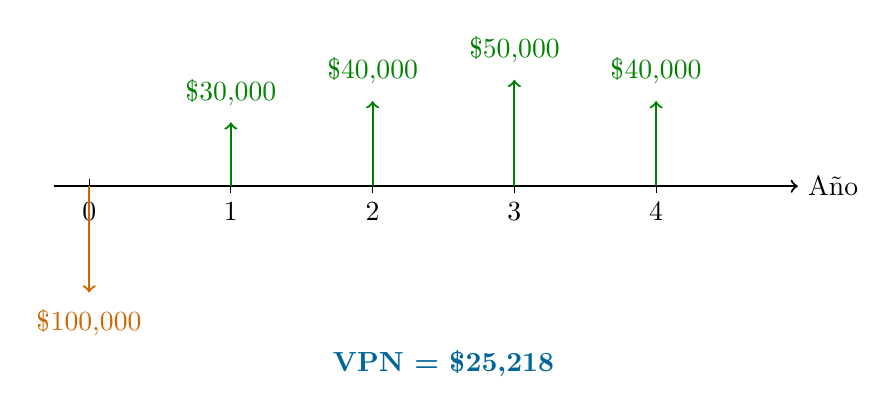
\begin{tikzpicture}[scale=0.9]
            % Línea de tiempo
            \draw[thick, ->] (-0.5,0) -- (10,0) node[right] {Año};

            % Marcas
            \foreach \x/\label in {0/0, 2/1, 4/2, 6/3, 8/4} {
                \draw (\x,0.1) -- (\x,-0.1) node[below] {\label};
            }

            % Inversión inicial
            \draw[thick, ->, accentorange] (0,0) -- (0,-1.5);
            \node[accentorange, below] at (0,-1.6) {\$100,000};

            % Flujos positivos
            \draw[thick, ->, accentgreen] (2,0) -- (2,0.9);
            \node[accentgreen, above] at (2,1.0) {\$30,000};

            \draw[thick, ->, accentgreen] (4,0) -- (4,1.2);
            \node[accentgreen, above] at (4,1.3) {\$40,000};

            \draw[thick, ->, accentgreen] (6,0) -- (6,1.5);
            \node[accentgreen, above] at (6,1.6) {\$50,000};

            \draw[thick, ->, accentgreen] (8,0) -- (8,1.2);
            \node[accentgreen, above] at (8,1.3) {\$40,000};

            % VPN
            \node[primaryblue] at (5,-2.5) {\textbf{VPN = \$25,218}};
        \end{tikzpicture}
    \end{center}
\end{frame}

\begin{frame}{VPN como Función de la Tasa}
    \begin{center}
        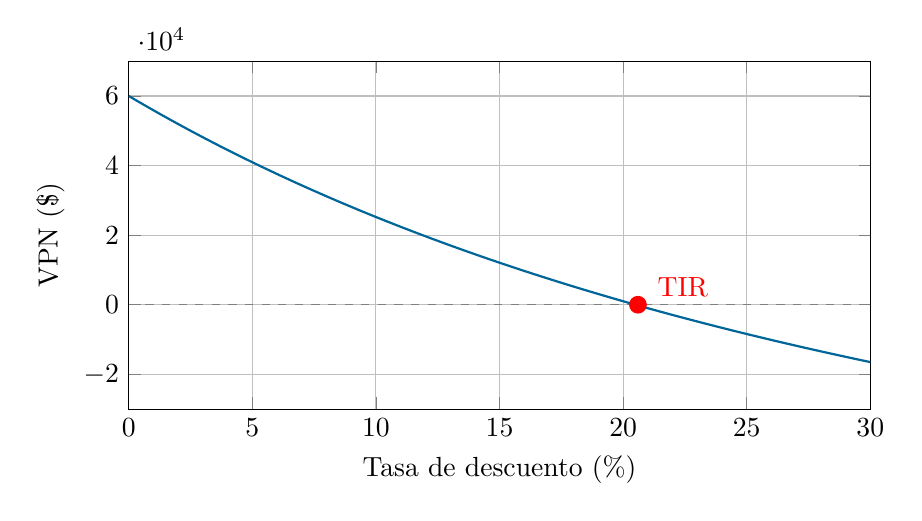
\begin{tikzpicture}
            \begin{axis}[
                xlabel={Tasa de descuento (\%)},
                ylabel={VPN (\$)},
                xmin=0, xmax=30,
                ymin=-30000, ymax=70000,
                grid=major,
                width=11cm,
                height=6cm
            ]
            % VPN del ejemplo
            \addplot[color=primaryblue, thick, domain=0:30, samples=50]
                {30000/(1+x/100) + 40000/(1+x/100)^2 + 50000/(1+x/100)^3 + 40000/(1+x/100)^4 - 100000};

            % Línea en VPN = 0
            \addplot[color=gray, dashed] coordinates {(0,0) (30,0)};

            % TIR (aproximada)
            \addplot[only marks, mark=*, mark size=3pt, color=red] coordinates {(20.6,0)};
            \node[right] at (axis cs:21,5000) {\textcolor{red}{TIR}};
            \end{axis}
        \end{tikzpicture}
    \end{center}

    El VPN disminuye conforme aumenta la tasa de descuento.
\end{frame}

% ===========================================
% SECCIÓN 4: TASA INTERNA DE RETORNO (TIR)
% ===========================================
\section{Tasa Interna de Retorno (TIR)}

\begin{frame}{Definición de la TIR}
    \begin{block}{Tasa Interna de Retorno}
        La \textbf{TIR} es la tasa de descuento que hace que el VPN sea igual a cero:
        \[
        \boxed{\sum_{t=0}^{n} \frac{CF_t}{(1+TIR)^t} = 0}
        \]
        O equivalentemente:
        \[
        \sum_{t=1}^{n} \frac{CF_t}{(1+TIR)^t} = I_0
        \]
    \end{block}

    \pause
    \vspace{0.3cm}

    \begin{exampleblock}{Interpretación}
        La TIR es el \textbf{rendimiento porcentual} que genera el proyecto sobre el capital invertido.
    \end{exampleblock}
\end{frame}

\begin{frame}{Regla de Decisión de la TIR}
    \begin{block}{Criterio de Aceptación}
        Si $r$ es el costo de capital (tasa mínima requerida):
        \begin{itemize}
            \item \textbf{TIR > r}: Aceptar el proyecto
            \item \textbf{TIR < r}: Rechazar el proyecto
            \item \textbf{TIR = r}: Indiferente
        \end{itemize}
    \end{block}

    \pause
    \vspace{0.3cm}

    \begin{alertblock}{Relación con VPN}
        \begin{itemize}
            \item Si TIR > r, entonces VPN > 0
            \item Si TIR < r, entonces VPN < 0
            \item Si TIR = r, entonces VPN = 0
        \end{itemize}
    \end{alertblock}
\end{frame}

\begin{frame}{Cálculo de la TIR}
    \begin{alertblock}{No hay solución algebraica directa}
        La TIR se calcula por:
        \begin{itemize}
            \item Prueba y error / interpolación
            \item Calculadora financiera (HP 12C)
            \item Métodos numéricos (Newton-Raphson)
            \item Software (Excel, Python)
        \end{itemize}
    \end{alertblock}

    \pause
    \vspace{0.3cm}

    \textbf{Interpolación lineal:}

    Si conocemos $VPN_1 > 0$ a tasa $r_1$ y $VPN_2 < 0$ a tasa $r_2$:
    \[
    TIR \approx r_1 + \frac{VPN_1}{VPN_1 - VPN_2} \times (r_2 - r_1)
    \]
\end{frame}

\begin{frame}{Ejemplo: Cálculo de TIR por Interpolación}
    \begin{block}{Del ejemplo anterior}
        Inversión: \$100,000. Flujos: 30k, 40k, 50k, 40k.
    \end{block}

    \pause
    \vspace{0.2cm}

    \textbf{Probando tasas:}
    \begin{itemize}
        \item $r = 10\%$: $VPN = \$25,218$ (positivo)
        \item $r = 20\%$: $VPN = \$2,662$ (positivo, cerca de cero)
        \item $r = 25\%$: $VPN = -\$8,480$ (negativo)
    \end{itemize}

    \pause
    \textbf{Interpolando entre 20\% y 25\%:}
    \begin{align*}
        TIR &\approx 20\% + \frac{2,662}{2,662 - (-8,480)} \times (25\% - 20\%) \\
        &= 20\% + \frac{2,662}{11,142} \times 5\% = 20\% + 1.19\% = 21.19\%
    \end{align*}

    \pause
    \textbf{TIR $\approx$ 21\%} (exacto por métodos numéricos: 20.6\%)
\end{frame}

% ===========================================
% SECCIÓN 5: CONFLICTOS VPN vs TIR
% ===========================================
\section{Conflictos entre VPN y TIR}

\begin{frame}{¿Cuándo VPN y TIR dan respuestas diferentes?}
    \textbf{Para un solo proyecto:}

    VPN y TIR siempre dan la misma decisión (aceptar/rechazar).

    \pause
    \vspace{0.5cm}

    \textbf{Para proyectos mutuamente excluyentes:}

    VPN y TIR pueden dar \textbf{rankings diferentes}.

    \pause
    \vspace{0.3cm}

    \begin{alertblock}{Causas del conflicto}
        \begin{enumerate}
            \item Diferente escala (montos de inversión)
            \item Diferente temporalidad de flujos
            \item Diferente vida útil
        \end{enumerate}
    \end{alertblock}
\end{frame}

\begin{frame}{Ejemplo: Conflicto por Escala}
    \begin{block}{Dos proyectos mutuamente excluyentes}
        \begin{center}
        \begin{tabular}{@{}lccc@{}}
            \toprule
            & Inversión & Flujo Año 1 & TIR \\
            \midrule
            Proyecto A & \$10,000 & \$12,000 & 20\% \\
            Proyecto B & \$50,000 & \$57,500 & 15\% \\
            \bottomrule
        \end{tabular}
        \end{center}
    \end{block}

    \pause
    \vspace{0.3cm}

    \textbf{Si el costo de capital es 10\%:}
    \begin{align*}
        VPN_A &= \frac{12,000}{1.10} - 10,000 = \$909 \\
        VPN_B &= \frac{57,500}{1.10} - 50,000 = \$2,273
    \end{align*}

    \pause
    \textbf{Conflicto:} TIR favorece A (20\% > 15\%), pero VPN favorece B (\$2,273 > \$909).

    \textbf{Decisión correcta:} Elegir B (mayor creación de valor).
\end{frame}

\begin{frame}{Ejemplo: Conflicto por Temporalidad}
    \begin{block}{Proyectos con diferente patrón de flujos}
        \begin{center}
        \scriptsize
        \begin{tabular}{@{}lcccccc@{}}
            \toprule
            & $I_0$ & Año 1 & Año 2 & Año 3 & Año 4 & TIR \\
            \midrule
            Proyecto X & -100 & 60 & 50 & 40 & 20 & 25.5\% \\
            Proyecto Y & -100 & 20 & 40 & 50 & 80 & 22.8\% \\
            \bottomrule
        \end{tabular}
        \end{center}
    \end{block}

    \pause
    \vspace{0.3cm}

    \textbf{VPN a diferentes tasas:}
    \begin{center}
    \scriptsize
    \begin{tabular}{@{}lcc@{}}
        \toprule
        Tasa & VPN$_X$ & VPN$_Y$ \\
        \midrule
        5\% & \$54.5 & \$66.7 \\
        15\% & \$28.5 & \$27.8 \\
        20\% & \$18.3 & \$14.7 \\
        \bottomrule
    \end{tabular}
    \end{center}

    A tasas bajas, Y es mejor (VPN mayor). A tasas altas, X es mejor.
\end{frame}

\begin{frame}{Tasa de Cruce (Crossover Rate)}
    \begin{center}
        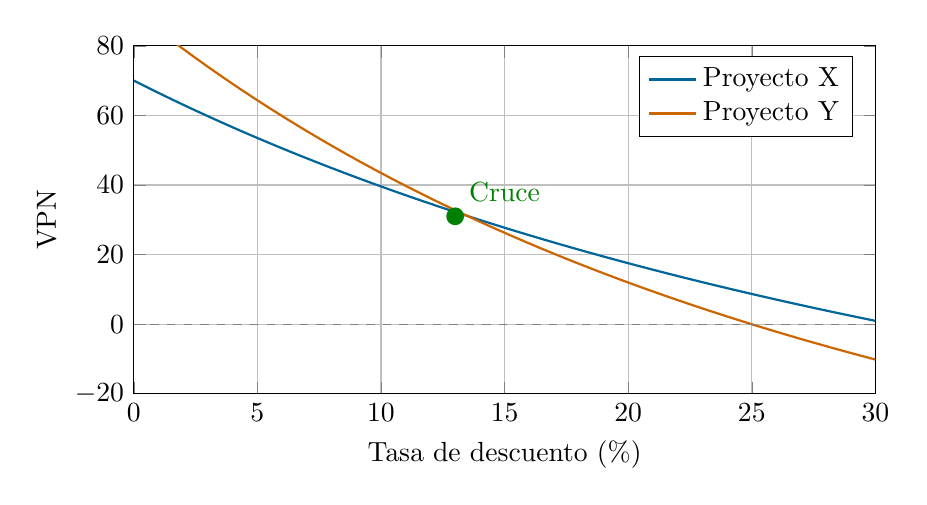
\begin{tikzpicture}
            \begin{axis}[
                xlabel={Tasa de descuento (\%)},
                ylabel={VPN},
                xmin=0, xmax=30,
                ymin=-20, ymax=80,
                grid=major,
                width=11cm,
                height=6cm,
                legend pos=north east
            ]
            % Proyecto X
            \addplot[color=primaryblue, thick, domain=0:30, samples=50]
                {60/(1+x/100) + 50/(1+x/100)^2 + 40/(1+x/100)^3 + 20/(1+x/100)^4 - 100};
            \addlegendentry{Proyecto X}

            % Proyecto Y
            \addplot[color=accentorange, thick, domain=0:30, samples=50]
                {20/(1+x/100) + 40/(1+x/100)^2 + 50/(1+x/100)^3 + 80/(1+x/100)^4 - 100};
            \addlegendentry{Proyecto Y}

            % Línea VPN = 0
            \addplot[color=gray, dashed] coordinates {(0,0) (30,0)};

            % Punto de cruce
            \addplot[only marks, mark=*, mark size=3pt, color=accentgreen] coordinates {(13,31)};
            \node at (axis cs:15,38) {\textcolor{accentgreen}{Cruce}};
            \end{axis}
        \end{tikzpicture}
    \end{center}

    Por debajo del cruce, Y es mejor. Por encima, X es mejor.
\end{frame}

\begin{frame}{Regla de Oro: Siempre Usar VPN}
    \begin{alertblock}{Recomendación}
        En caso de conflicto entre VPN y TIR, \textbf{siempre} usar el criterio del VPN.
    \end{alertblock}

    \pause
    \vspace{0.3cm}

    \textbf{Razones:}
    \begin{enumerate}
        \item VPN mide directamente la creación de riqueza
        \item TIR asume reinversión a la misma TIR (supuesto irrealista)
        \item VPN asume reinversión al costo de capital (más realista)
        \item VPN es aditivo (VPN de A + B = VPN$_A$ + VPN$_B$)
    \end{enumerate}

    \pause
    \vspace{0.3cm}

    \begin{exampleblock}{Cuándo usar TIR}
        La TIR es útil para \textbf{comunicar} el rendimiento de un proyecto, pero no para tomar decisiones entre alternativas.
    \end{exampleblock}
\end{frame}

% ===========================================
% SECCIÓN 6: PROBLEMAS CON LA TIR
% ===========================================
\section{Problemas con la TIR}

\begin{frame}{TIR Múltiple}
    \begin{block}{El problema}
        Cuando los flujos cambian de signo más de una vez, puede existir \textbf{más de una TIR}.
    \end{block}

    \pause
    \vspace{0.3cm}

    \textbf{Ejemplo:}

    $CF_0 = -100$, $CF_1 = +230$, $CF_2 = -132$

    \pause
    \begin{align*}
        -100 + \frac{230}{(1+r)} + \frac{-132}{(1+r)^2} = 0
    \end{align*}

    Resolviendo: $TIR_1 = 10\%$ y $TIR_2 = 20\%$

    \pause
    \vspace{0.3cm}

    \begin{alertblock}{¿Cuál usar?}
        ¡Ninguna tiene significado económico claro! Usar VPN en estos casos.
    \end{alertblock}
\end{frame}

\begin{frame}{Visualización de TIR Múltiple}
    \begin{center}
        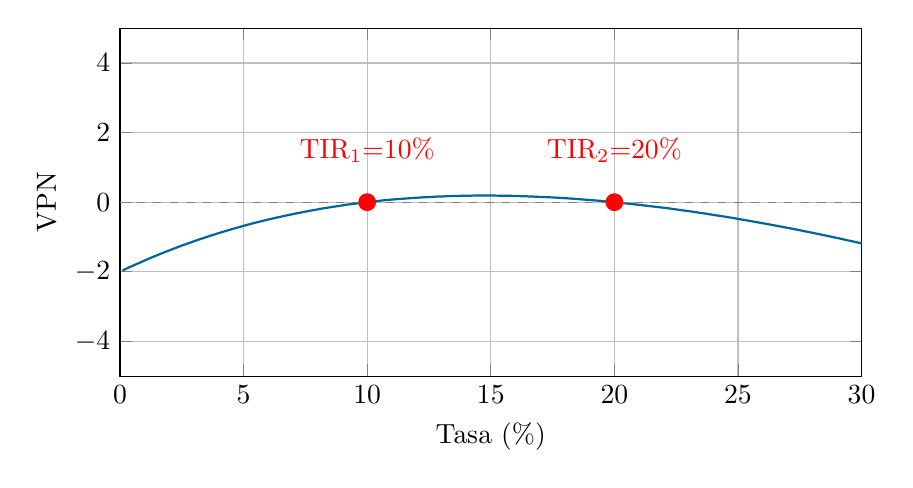
\begin{tikzpicture}
            \begin{axis}[
                xlabel={Tasa (\%)},
                ylabel={VPN},
                xmin=0, xmax=30,
                ymin=-5, ymax=5,
                grid=major,
                width=11cm,
                height=6cm
            ]
            \addplot[color=primaryblue, thick, domain=0.1:30, samples=100]
                {-100 + 230/(1+x/100) - 132/(1+x/100)^2};

            \addplot[color=gray, dashed] coordinates {(0,0) (30,0)};

            % Dos TIRs
            \addplot[only marks, mark=*, mark size=3pt, color=red] coordinates {(10,0) (20,0)};
            \node at (axis cs:10,1.5) {\textcolor{red}{TIR$_1$=10\%}};
            \node at (axis cs:20,1.5) {\textcolor{red}{TIR$_2$=20\%}};
            \end{axis}
        \end{tikzpicture}
    \end{center}

    La curva de VPN cruza el eje horizontal dos veces.
\end{frame}

\begin{frame}{Regla de los Signos de Descartes}
    \begin{alertblock}{Número máximo de TIRs}
        El número de TIRs reales positivas es \textbf{a lo más} igual al número de cambios de signo en los flujos.
    \end{alertblock}

    \pause
    \vspace{0.3cm}

    \textbf{Ejemplos:}
    \begin{itemize}
        \item $(-,+,+,+)$: 1 cambio de signo $\to$ máximo 1 TIR
        \item $(-,+,+,-)$: 2 cambios de signo $\to$ máximo 2 TIRs
        \item $(-,+,-,+)$: 3 cambios de signo $\to$ máximo 3 TIRs
    \end{itemize}

    \pause
    \vspace{0.3cm}

    \begin{exampleblock}{Proyectos ``normales''}
        Proyectos con inversión inicial negativa y flujos positivos posteriores ($-,+,+,...,+$) tienen exactamente \textbf{una} TIR.
    \end{exampleblock}
\end{frame}

\begin{frame}{Proyecto sin TIR}
    \begin{block}{Caso especial}
        Algunos proyectos no tienen TIR real (la curva de VPN nunca cruza cero).
    \end{block}

    \pause
    \vspace{0.3cm}

    \textbf{Ejemplo:}

    $CF_0 = +100$, $CF_1 = -300$, $CF_2 = +250$

    \pause
    \begin{center}
        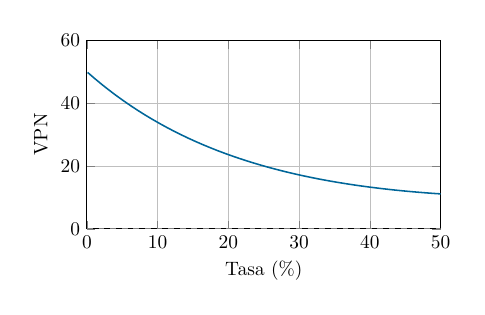
\begin{tikzpicture}[scale=0.7]
            \begin{axis}[
                xlabel={Tasa (\%)},
                ylabel={VPN},
                xmin=0, xmax=50,
                ymin=0, ymax=60,
                grid=major,
                width=8cm,
                height=5cm
            ]
            \addplot[color=primaryblue, thick, domain=0.1:50, samples=50]
                {100 - 300/(1+x/100) + 250/(1+x/100)^2};

            \addplot[color=gray, dashed] coordinates {(0,0) (50,0)};
            \end{axis}
        \end{tikzpicture}
    \end{center}

    VPN siempre positivo (buen proyecto), pero no hay TIR.
\end{frame}

% ===========================================
% SECCIÓN 7: TRUCOS Y HP 12C
% ===========================================
\section{Trucos de Estimación Mental}

\begin{frame}{Estimación Rápida del VPN}
    \begin{alertblock}{Para flujos uniformes}
        Si los flujos son aproximadamente constantes:
        \[
        VPN \approx CF \times PVIFA_{r,n} - I_0
        \]
    \end{alertblock}

    \pause
    \vspace{0.3cm}

    \textbf{Ejemplo:}

    Inversión \$100,000, flujos de \$30,000 por 5 años, tasa 10\%.

    \begin{align*}
        VPN &\approx 30,000 \times 3.79 - 100,000 \\
        &= 113,700 - 100,000 = \$13,700
    \end{align*}

    (PVIFA de la tabla de la Sesión 5)
\end{frame}

\begin{frame}{Payback como Indicador de TIR}
    \begin{alertblock}{Relación aproximada}
        Para proyectos con flujos uniformes:
        \[
        TIR \approx \frac{1}{\text{Payback}} \times \text{factor de ajuste}
        \]

        El factor es cercano a 1.5-2 para proyectos de 5-10 años.
    \end{alertblock}

    \pause
    \vspace{0.3cm}

    \textbf{Ejemplo:}

    Inversión \$100,000, flujos de \$25,000/año.

    Payback = $100,000 / 25,000 = 4$ años

    TIR aproximada $\approx 1/4 \times 1.7 \approx 42\%$

    (Esto es solo una estimación gruesa)
\end{frame}

\section{Calculadora HP 12C}

\begin{frame}{HP 12C: Cálculo de VPN}
    \begin{block}{Problema}
        Inversión: \$50,000. Flujos: Año 1: \$15,000, Año 2: \$20,000, Año 3: \$25,000. Tasa: 12\%.
    \end{block}

    \pause
    \vspace{0.2cm}

    \begin{center}
    \scriptsize
    \begin{tabular}{@{}lll@{}}
        \toprule
        \textbf{Teclas} & \textbf{Display} & \textbf{Descripción} \\
        \midrule
        \texttt{f CLX} & 0.00 & Limpiar \\
        \texttt{50000 CHS g CF$_0$} & -50,000 & Inversión inicial \\
        \texttt{15000 g CF$_j$} & 15,000 & Flujo año 1 \\
        \texttt{20000 g CF$_j$} & 20,000 & Flujo año 2 \\
        \texttt{25000 g CF$_j$} & 25,000 & Flujo año 3 \\
        \texttt{12 i} & 12 & Tasa de descuento \\
        \texttt{f NPV} & \textbf{1,103.19} & VPN \\
        \bottomrule
    \end{tabular}
    \end{center}

    \pause
    VPN = \$1,103.19 > 0, aceptar el proyecto.
\end{frame}

\begin{frame}{HP 12C: Cálculo de TIR}
    \textbf{Continuando del ejemplo anterior...}

    \pause
    \vspace{0.3cm}

    \begin{center}
    \begin{tabular}{@{}lll@{}}
        \toprule
        \textbf{Teclas} & \textbf{Display} & \textbf{Descripción} \\
        \midrule
        \texttt{f IRR} & \textbf{13.67} & TIR del proyecto \\
        \bottomrule
    \end{tabular}
    \end{center}

    \pause
    \vspace{0.3cm}

    \textbf{TIR = 13.67\%}

    Como TIR (13.67\%) > costo de capital (12\%), aceptar el proyecto.

    \pause
    \vspace{0.3cm}

    \begin{exampleblock}{Verificación}
        Ambos criterios coinciden: VPN > 0 y TIR > r
    \end{exampleblock}
\end{frame>

\begin{frame}{HP 12C: Flujos con Repetición}
    \begin{block}{Problema}
        Inversión: \$100,000. Flujos: \$30,000 por 5 años. Tasa: 10\%.
    \end{block}

    \pause
    \vspace{0.2cm}

    \begin{center}
    \scriptsize
    \begin{tabular}{@{}lll@{}}
        \toprule
        \textbf{Teclas} & \textbf{Display} & \textbf{Descripción} \\
        \midrule
        \texttt{f CLX} & 0.00 & Limpiar \\
        \texttt{100000 CHS g CF$_0$} & -100,000 & Inversión \\
        \texttt{30000 g CF$_j$} & 30,000 & Flujo periódico \\
        \texttt{5 g N$_j$} & 5 & Se repite 5 veces \\
        \texttt{10 i} & 10 & Tasa \\
        \texttt{f NPV} & \textbf{13,723.60} & VPN \\
        \texttt{f IRR} & \textbf{15.24} & TIR \\
        \bottomrule
    \end{tabular}
    \end{center}

    La tecla \texttt{g N$_j$} indica cuántas veces se repite el último flujo.
\end{frame}

% ===========================================
% SECCIÓN 8: EJERCICIOS PRÁCTICOS
% ===========================================
\section{Ejercicios Prácticos}

\begin{frame}{Ejercicio 1: VPN Básico}
    \begin{block}{Problema}
        Una empresa considera comprar equipo por \$200,000. Genera ahorros de \$60,000 anuales por 5 años. Al final, se vende en \$30,000. Si el costo de capital es 15\%, ¿conviene?
    \end{block}

    \pause
    \vspace{0.2cm}

    \textbf{Solución:}
    \begin{align*}
        VPN &= 60,000 \times \frac{1-(1.15)^{-5}}{0.15} + \frac{30,000}{(1.15)^5} - 200,000 \\[0.2cm]
        &= 60,000 \times 3.3522 + 30,000 \times 0.4972 - 200,000 \\[0.2cm]
        &= 201,132 + 14,916 - 200,000 = \$16,048
    \end{align*}

    \pause
    VPN > 0, por lo tanto \textbf{sí conviene}.
\end{frame}

\begin{frame}{Ejercicio 2: TIR por Interpolación}
    \begin{block}{Problema}
        Proyecto: Inversión \$80,000, flujos de \$25,000 por 4 años. Estimar la TIR.
    \end{block}

    \pause
    \vspace{0.2cm}

    \textbf{Probando tasas:}
    \begin{itemize}
        \item $r = 10\%$: $VPN = 25,000 \times 3.170 - 80,000 = -\$751$ (negativo)
        \item $r = 8\%$: $VPN = 25,000 \times 3.312 - 80,000 = +\$2,800$ (positivo)
    \end{itemize}

    \pause
    \textbf{Interpolando:}
    \begin{align*}
        TIR &\approx 8\% + \frac{2,800}{2,800 + 751} \times (10\% - 8\%) \\
        &= 8\% + 0.79 \times 2\% = 9.58\%
    \end{align*}

    \textbf{TIR $\approx$ 9.6\%}
\end{frame}

\begin{frame}{Ejercicio 3: Proyectos Excluyentes}
    \begin{block}{Problema}
        Proyecto A: -100, +50, +50, +50 (TIR = 23.4\%)

        Proyecto B: -100, +10, +30, +100 (TIR = 17.7\%)

        Costo de capital: 10\%. ¿Cuál elegir?
    \end{block}

    \pause
    \vspace{0.2cm}

    \textbf{Calculando VPN al 10\%:}
    \begin{align*}
        VPN_A &= \frac{50}{1.1} + \frac{50}{1.1^2} + \frac{50}{1.1^3} - 100 = \$24.34 \\[0.2cm]
        VPN_B &= \frac{10}{1.1} + \frac{30}{1.1^2} + \frac{100}{1.1^3} - 100 = \$9.94
    \end{align*}

    \pause
    \textbf{TIR favorece A (23.4\% > 17.7\%)} \checkmark

    \textbf{VPN favorece A (\$24.34 > \$9.94)} \checkmark

    Ambos coinciden: elegir A.
\end{frame}

\begin{frame}{Ejercicio 4: Conflicto VPN-TIR}
    \begin{block}{Problema}
        Proyecto X: -1,000, +1,300. TIR = 30\%.

        Proyecto Y: -10,000, +12,000. TIR = 20\%.

        Costo de capital: 10\%. ¿Cuál elegir?
    \end{block}

    \pause
    \vspace{0.2cm}

    \textbf{VPN al 10\%:}
    \begin{align*}
        VPN_X &= 1,300/1.1 - 1,000 = \$181.82 \\
        VPN_Y &= 12,000/1.1 - 10,000 = \$909.09
    \end{align*}

    \pause
    \textbf{TIR favorece X (30\% > 20\%)}

    \textbf{VPN favorece Y (\$909 > \$182)} \checkmark

    \textbf{Decisión correcta:} Elegir Y (mayor creación de valor).
\end{frame>

% ===========================================
% SECCIÓN 9: PYTHON
% ===========================================
\section{Python con numpy-financial}

\begin{frame}[fragile]{Python: Cálculo de VPN y TIR}
    \begin{lstlisting}[style=pythonstyle]
import numpy_financial as npf

# Definir flujos de caja
flujos = [-100000, 30000, 40000, 50000, 40000]
tasa = 0.10

# Calcular VPN
# npf.npv calcula VP de flujos desde periodo 1
# Debemos ajustar para incluir el flujo en t=0
vpn = npf.npv(tasa, flujos[1:]) + flujos[0]
print(f"VPN: ${vpn:,.2f}")

# Calcular TIR
tir = npf.irr(flujos)
print(f"TIR: {tir*100:.2f}%")

# Verificacion: VPN a la TIR debe ser 0
vpn_tir = npf.npv(tir, flujos[1:]) + flujos[0]
print(f"VPN a la TIR: ${vpn_tir:.2f}")
    \end{lstlisting}
\end{frame}

\begin{frame}[fragile]{Python: Perfil de VPN}
    \begin{lstlisting}[style=pythonstyle]
import numpy as np
import matplotlib.pyplot as plt
import numpy_financial as npf

flujos = [-100000, 30000, 40000, 50000, 40000]
tasas = np.linspace(0.01, 0.30, 50)

vpns = [npf.npv(r, flujos[1:]) + flujos[0] for r in tasas]

plt.figure(figsize=(10, 5))
plt.plot(tasas*100, vpns, 'b-', linewidth=2)
plt.axhline(y=0, color='gray', linestyle='--')
plt.xlabel('Tasa de descuento (%)')
plt.ylabel('VPN ($)')
plt.title('Perfil de VPN del Proyecto')
plt.grid(True)

# Marcar TIR
tir = npf.irr(flujos)
plt.axvline(x=tir*100, color='red', linestyle='--', label=f'TIR = {tir*100:.1f}%')
plt.legend()
plt.savefig('perfil_vpn.png')
    \end{lstlisting}
\end{frame}

\begin{frame}[fragile]{Python: Comparar Proyectos}
    \begin{lstlisting}[style=pythonstyle]
import numpy_financial as npf
import numpy as np

proyectos = {
    'A': [-100, 50, 50, 50],
    'B': [-100, 10, 30, 100]
}

print("Proyecto | TIR    | VPN@10%")
print("-" * 35)

for nombre, flujos in proyectos.items():
    tir = npf.irr(flujos)
    vpn = npf.npv(0.10, flujos[1:]) + flujos[0]
    print(f"{nombre:8} | {tir*100:5.1f}% | ${vpn:,.2f}")

# Encontrar tasa de cruce
flujos_diff = [a-b for a,b in zip(proyectos['A'], proyectos['B'])]
cruce = npf.irr(flujos_diff)
print(f"\nTasa de cruce: {cruce*100:.2f}%")
    \end{lstlisting}
\end{frame}

% ===========================================
% SECCIÓN 10: RESUMEN Y TAREA
% ===========================================
\section{Resumen y Tarea}

\begin{frame}{Resumen de Fórmulas}
    \textbf{Valor Presente Neto:}
    \[
    VPN = \sum_{t=1}^{n} \frac{CF_t}{(1+r)^t} - I_0
    \]

    \textbf{Tasa Interna de Retorno:}
    \[
    \sum_{t=0}^{n} \frac{CF_t}{(1+TIR)^t} = 0
    \]

    \textbf{Interpolación para TIR:}
    \[
    TIR \approx r_1 + \frac{VPN_1}{VPN_1 - VPN_2} \times (r_2 - r_1)
    \]
\end{frame}

\begin{frame}{Conceptos Clave}
    \begin{enumerate}
        \item \textbf{VPN} mide la creación de valor en pesos
        \item \textbf{TIR} mide el rendimiento porcentual del proyecto
        \item Regla VPN: Aceptar si $VPN > 0$
        \item Regla TIR: Aceptar si $TIR > r$
        \item VPN y TIR pueden \textbf{conflictar} en proyectos excluyentes
        \item En caso de conflicto, \textbf{usar VPN}
        \item TIR puede ser \textbf{múltiple} o no existir
        \item HP 12C: \texttt{g CF$_j$}, \texttt{f NPV}, \texttt{f IRR}
    \end{enumerate}
\end{frame}

\begin{frame}{Tarea para la Próxima Sesión}
    \begin{enumerate}
        \item \textbf{Cálculo:} Proyecto con inversión \$150,000, flujos de \$45,000 por 5 años, tasa 12\%. Calcular VPN y TIR.

        \vspace{0.3cm}

        \item \textbf{Comparación:} Dos proyectos con inversión \$50,000 cada uno. A genera \$20,000/año por 4 años. B genera \$10,000, \$15,000, \$20,000, \$25,000. ¿Cuál elegir al 8\%?

        \vspace{0.3cm}

        \item \textbf{HP 12C:} Practica ingresando flujos irregulares y calculando VPN/TIR.

        \vspace{0.3cm}

        \item \textbf{Python:} Grafica el perfil de VPN de dos proyectos y encuentra la tasa de cruce.
    \end{enumerate}
\end{frame}

% ===========================================
% CIERRE
% ===========================================

\begin{frame}
    \begin{center}
        \Huge \textcolor{primaryblue}{\textbf{¿Preguntas?}}

        \vspace{1cm}
        \Large Próxima Sesión:\\
        \textbf{Valuación de Acciones e Integración}

        \vspace{0.5cm}
        \normalsize Semana 5, Clase 2
    \end{center}
\end{frame}

\end{document}
